
\documentclass[chaptersright]{informeutn}
\usepackage{circuitikz}
\usepackage{pgfplots}
\usepackage[siunitx]



\title{%
\setlength{\headwidth}{\textwidth} % Hace que el encabezado tenga el mismo ancho que el contenido
\setlength{\headheight}{15pt}  % Ajusta la altura del encabezado
\setlength{\headsep}{10pt}     % Ajusta la separación entre el encabezado y el contenido
  \fontsize{25}{0}\selectfont Universidad Tecnológica Nacional \\
  \fontsize{22}{30}\selectfont Dispositivos Electronicos I \\
  \fontsize{20}{25}\selectfont Trabajo Practico N°
}
\author{
  Santino Noccetti - 405927\\
  Franco Palombo - 401910\\
}
\date{1 / 1 / 2025}
% Datos del informe
\materia{Dispositivos Electronicos}
\titulo{Trabajo Práctico}
\comision{3R2}
\autores{
          Santino Noccetti, 405927 - Coordinador\\
          Franco Palombo, 401910 - Documentador/Operario}
\fecha{01/01/2001}

\begin{document}

  \maketitle

  \myemptypage

  \tableofcontents
  \setcounter{page}{1}
  \thispagestyle{plain}

  \myemptypage

  \chapter{Introduccion}
    En este trabajo practico se divide en el analisis de dos componentes. Por un lado en la simulacion del diodo rectificador, se busca visualizar el comportamiento de este y la curva caracteristica para asi comparar el codo de conmutacion entre el estado de bloqueo y conduccion que nos presenta el fabricante, luego armar un circuito en el laboratorio para poder medir y corroborar lo visto en el simulador. Ademas se incluye en la simulacion el factor de la temperatura, para poder ver como afecta al comportamiento.

    
    Luego se propone un circuito con diodos Zener en CA, para ello se nos exige utilizar el simulador LTspice para visualizar su uso para limitar las excursiones de voltaje a niveles deseados. Luego en el laboratorio se nos pide armar el mismo circuito para poder visualizar y analizar su uso como recortadores.
  \part{Curva caracteristica del diodo}
    \chapter{Actividad de simulacion}
        \section{Polarizacion en directa}
            \subsection{Diodo de silicio}
                A continuacion se presenta el circuito utilizado en LTspice para visualizar la curva caracteristica del diodo de Silicio.
    
    
                La configuracion utilizada fue:
                \begin{itemize}
                    \item Una fuente DC que realiza un barrido lineal de 100$mV$ desde -2 $V$ hasta los 10 $V$ 
                    \item Resistencia de 1$k$
                    \item Diodo 1N4007
                \end{itemize}
    
    
    
                \begin{figure}[h]
                    \centering
                    \begin{minipage}{0.7\textwidth}
                    \centering
                    \begin{circuitikz}[american voltages]
                         % nodos
                        \draw
                            (0, -1) to [V=$V_1$, on grid, invert]                   (0, 3)
                            to [short, -, i>^=$I_t$, on grid]               (1, 3)
                            to [R=$R_1$, v=$V_{R_1}$, on grid]              (4, 3)
                            to [short, -, on grid]                         (5, 3)
                            to [D=$1N4007$, v=$V_{D}$, on grid]              (5, -1)
                            to [short, -, on grid]                         (5, -1)
                            to [short, -, on grid]                          (0, -1)
                
                
                
                             ;
                    \end{circuitikz}
                \end{minipage}
                \centering
                \caption{Circuito con diodo de silicio}
                \end{figure}
    
                \newpage
                
                Comparacion del grafico obtenido en el simulador con el proporcionado en la hoja de datos del fabricante Diodes Incorporated:
      
    
                \begin{figure}[!h]
                    \centering
                    \begin{minipage}[b]{0.4\textwidth}
                        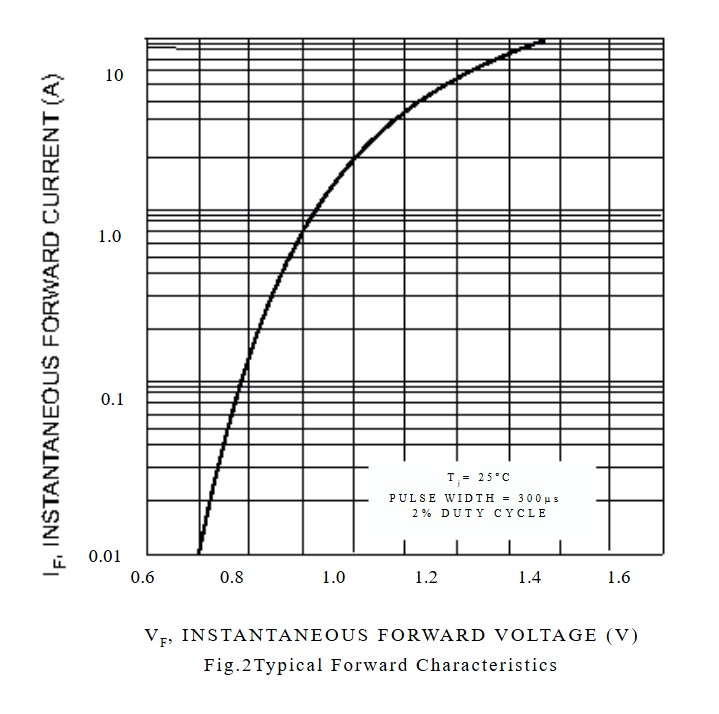
\includegraphics[width=1.1\linewidth]{pictures/Curva_Datash_Si.jpg}
                        \caption{Grafico de la curva del simulador}
                    \end{minipage}
                    \hfill
                    \begin{minipage}[b]{0.4\textwidth}
                        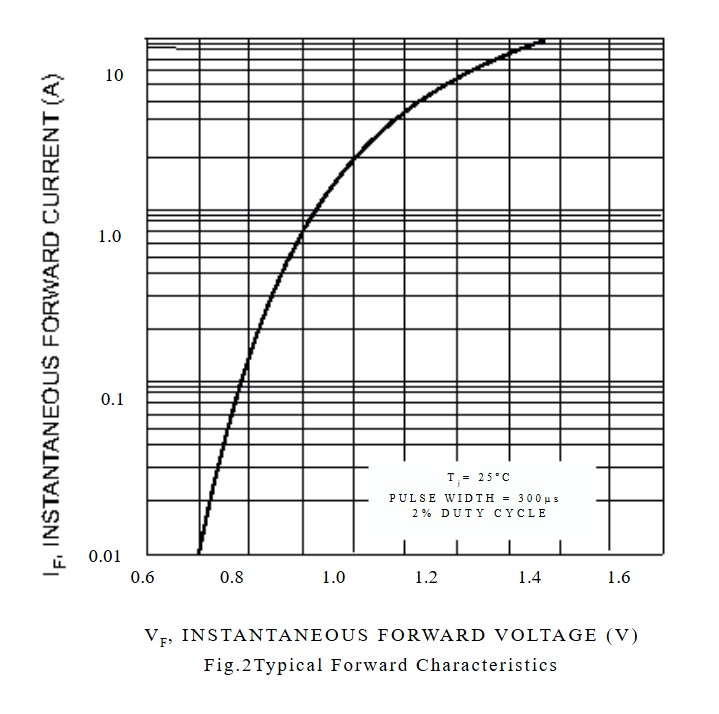
\includegraphics[width=1.1\linewidth]{pictures/Curva_Datash_Si.jpg}
                        \caption{Grafico de la curva del Datasheet}
                    \end{minipage}
                \end{figure}
    
                \subsubsection{Conclusion}
    
                    En ambos graficos se puede observar el comportamiento del diodo cuando esta conectado en directa, si bien la que nos proporciona el datasheet esta en escala logaritmica para poder mostrar bien desde los $nA$ hasta los $A$ pero no quita que ambos nos muestren los mismo. En la simulacion se logra observar el "codo de conmutacion" alrededor de los 0.6$V$ para luego entrar en estado de conduccion y permitir el paso de corriente corroborando asi la grafica del fabricante.
    
                \newpage
                
            \subsection{Diodo de Germanio}
            
                A continuacion se presenta el circuito utilizado en LTspice para visualizar la curva caracteristica del diodo de Germanio.
    
    
                La configuracion utilizada fue:
                \begin{itemize}
                    \item Una fuente DC que realiza un barrido lineal de 100$mV$ desde -2 $V$ hasta los 10 $V$ 
                    \item Resistencia de 1$k$
                    \item Diodo 1N60
                \end{itemize}
            
                \begin{figure}[h]
                    \centering
                    \begin{minipage}{0.7\textwidth}
                        \centering
                        \begin{circuitikz}[american voltages]
                            % nodos
                            \draw
                                (0, -1) to [V=$V_1$, on grid, invert]          (0, 3)
                                to [short, -, i>^=$I_t$, on grid]              (1, 3)
                                to [R=$R_1$, v=$V_{R_1}$, on grid]             (4, 3)
                                to [short, -, on grid]                         (5, 3)
                                to [D=$1N60$, v=$V_{D}$, on grid]              (5, -1)
                                to [short, -, on grid]                         (5, -1)
                                to [short, -, on grid]                         (0, -1)
                
                
                
                            ;
                    \end{circuitikz}
                \end{minipage}
                \centering
                \caption{Circuito con diodo de Germanio}
                \end{figure}
                \newpage

                Comparacion del grafico obtenido en el simulador con el proporcionado en la hoja de datos del fabricante Diode Semiconductor Korea:

                \begin{figure}[!h]
                    \centering
                    \begin{minipage}[b]{0.4\textwidth}
                        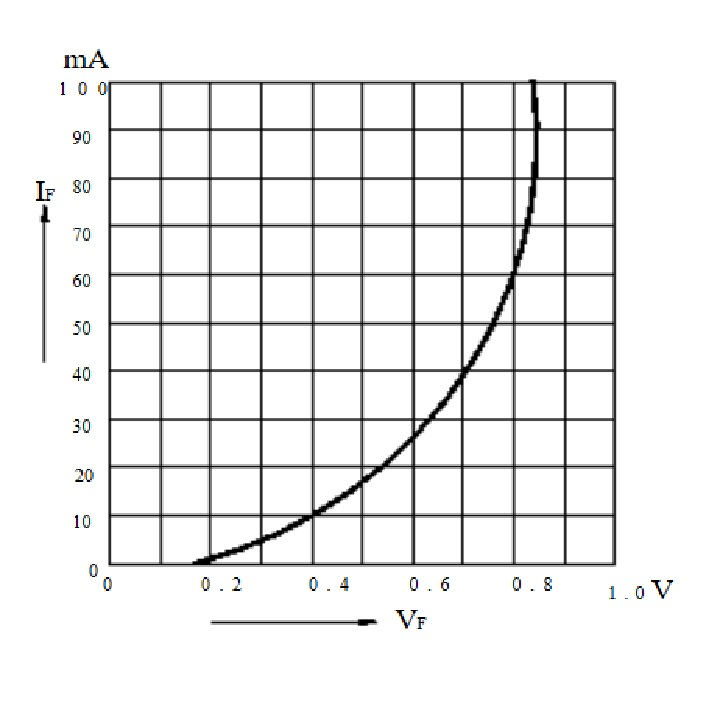
\includegraphics[width=1.1\linewidth]{pictures/Curva_Datash_Ge.jpg}
                        \caption{Grafico de la curva del simulador}
                    \end{minipage}
                    \hfill
                    \begin{minipage}[b]{0.4\textwidth}
                        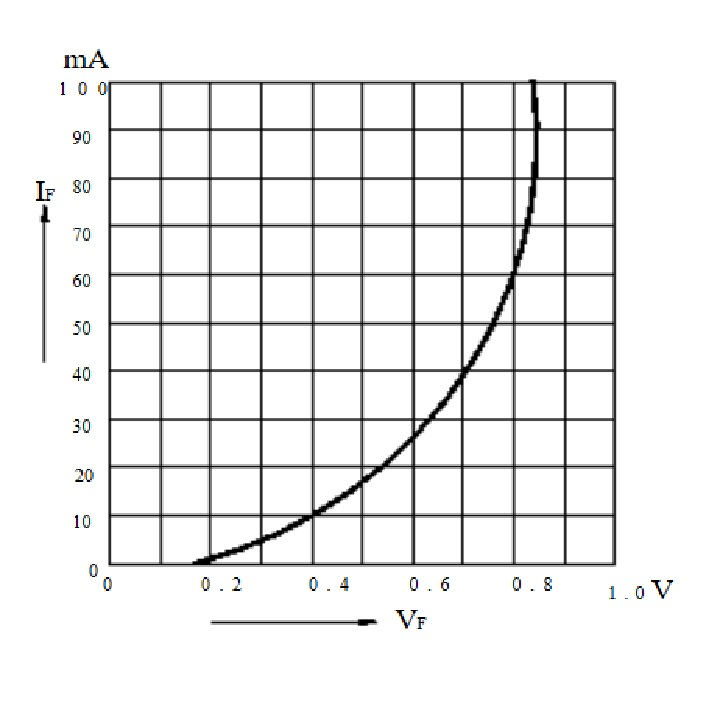
\includegraphics[width=1.1\linewidth]{pictures/Curva_Datash_Ge.jpg}
                        \caption{Grafico de la curva del Datasheet}
                    \end{minipage}
                \end{figure}

                \subsubsection{Conclusion}
                    Al igual que en el diodo de Silicio, este mantiene claras igualdades en la curva caracteristica del diodo comparandola con la hoja de datos del fabricante.
                    \newpage


                \subsection{Comparacion de ambas simulaciones}
                
                \begin{figure}[!h]
                    \centering
                    \begin{minipage}[b]{0.4\textwidth}
                        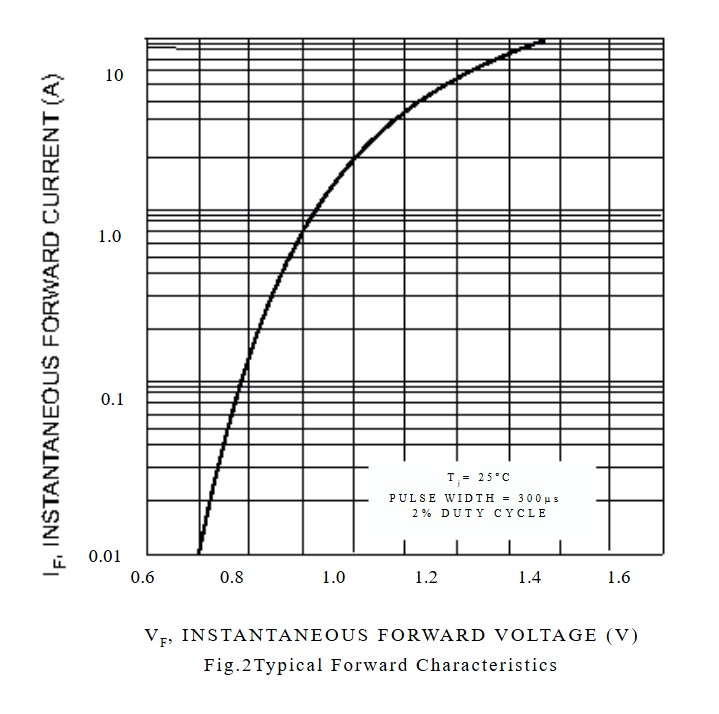
\includegraphics[width=1.1\linewidth]{pictures/Curva_Datash_Si.jpg}
                        \caption{Grafico de la curva del simulador}
                    \end{minipage}
                \end{figure}

                Cuando se observa de esta forma ambas curvas se logra apreciar una clara diferencia en cuanto al voltaje necesario para lograr poner los diodos en conduccion, siendo la de Germanio alrededor de los $0.2V$ y $0.3V$ mientras que el de Silicio se encuentra entre $0.6V$ y $0.7V$.Esta diferencia en el codo de conmutacion se debe principalmente a la diferencia de energia necesaria para que los electrones pasen de la banda de valencia a la banda de conduccion, a su vez tambien se le atribuye a que el Germanio posee mayor corriente de fuga, generando asi que la curva se pronuncie mucho antes que la del Silicio. Esto tiene implicaciones a la hora de elegir que tipo de diodo usar, ya que el de Germanio se utiliza para circuitos con poco voltaje, sin embargo, el de Silicio es el mas utilizado ya que posee menor corriente de fuga y mayor estabilidad a los cambios de temperatura.

                \newpage

                \section{Polarizacion en inversa}
                    \subsection{Diodo de silicio}
                        A continuacion se presenta el circuito utilizado en LTspice para visualizar la curva caracteristica del diodo de Silicio en inversa.
                        
                        \begin{itemize}
                            \item Una fuente DC que realiza un barrido lineal de 100$mV$ desde -2 $V$ hasta los 1200 $V$ 
                            \item Resistencia de 1$k$
                            \item Diodo 1N4007
                        \end{itemize}
                        \begin{figure}[h]
                            \centering
                            \begin{minipage}{0.7\textwidth}
                                \centering
                                \begin{circuitikz}[american voltages]
                                    % nodos
                                    \draw
                                        (0, -1) to [V=$V_1$, on grid, invert]          (0, 3)
                                        to [short, -, i>^=$I_t$, on grid]              (1, 3)
                                        to [R=$R_1$, v=$V_{R_1}$, on grid]             (4, 3)
                                        
                                        to [short, -, on grid]                         (5, 3)
                                        to [D=$1N4007$, v=$V_{D}$, on grid]            (5, -1)
                                        to [short, -, on grid]                         (5, -1)
                                        to [short, -, on grid]                         (0, -1)
                        
                        
                        
                                    ;
                            \end{circuitikz}
                        \end{minipage}
                        \centering
                        \caption{Circuito con diodo de Silicio en inversa}
                        \end{figure}           

                        \begin{figure}[!h]
                            \centering
                            \begin{minipage}[b]{0.4\textwidth}
                                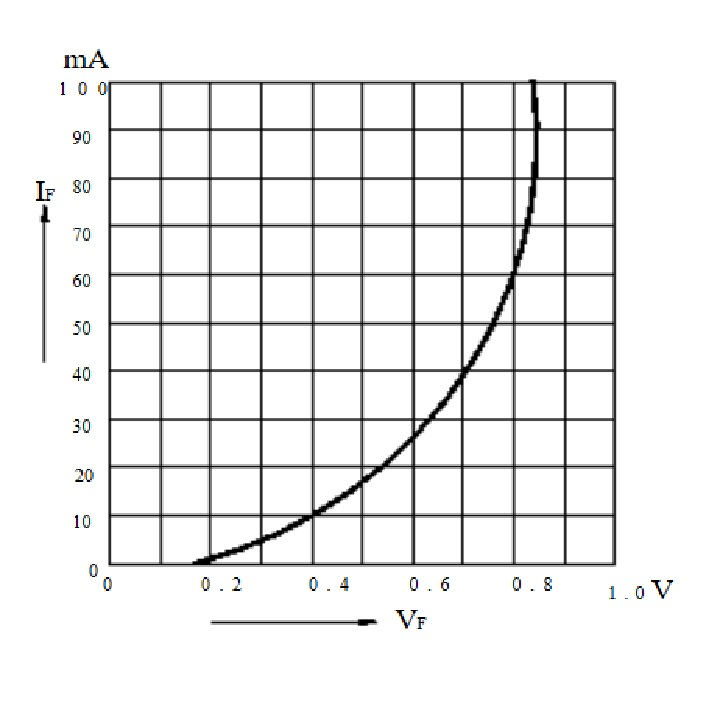
\includegraphics[width=1.1\linewidth]{pictures/Curva_Datash_Ge.jpg}
                                \caption{Grafico de la curva del diodo de Silicio en inversa}
                            \end{minipage}
                        \end{figure}

                    \newpage

                
                    \subsection{Diodo de Germanio}
                        A continuacion se presenta el circuito utilizado en LTspice para visualizar la curva caracteristica del diodo de Germanio en inversa.
                        
                        \begin{itemize}
                            \item Una fuente DC que realiza un barrido lineal de 100$mV$ desde -2 $V$ hasta los 45 $V$ 
                            \item Resistencia de 1$k$
                            \item Diodo 1N60
                        \end{itemize}
                        \begin{figure}[h]
                            \centering
                            \begin{minipage}{0.7\textwidth}
                                \centering
                                \begin{circuitikz}[american voltages]
                                    % nodos
                                    \draw
                                        (0, -1) to [V=$V_1$, on grid, invert]          (0, 3)
                                        to [short, -, i>^=$I_t$, on grid]              (1, 3)
                                        to [R=$R_1$, v=$V_{R_1}$, on grid]             (4, 3)
                                        
                                        to [short, -, on grid]                         (5, 3)
                                        to [D=$1N4007$, v=$V_{D}$, on grid]            (5, -1)
                                        to [short, -, on grid]                         (5, -1)
                                        to [short, -, on grid]                         (0, -1)
                        
                        
                        
                                    ;
                            \end{circuitikz}
                        \end{minipage}
                        \centering
                        \caption{Circuito con diodo de Germanio en inversa}
                        \end{figure}

                        \begin{figure}[!h]
                            \centering
                            \begin{minipage}[b]{0.4\textwidth}
                                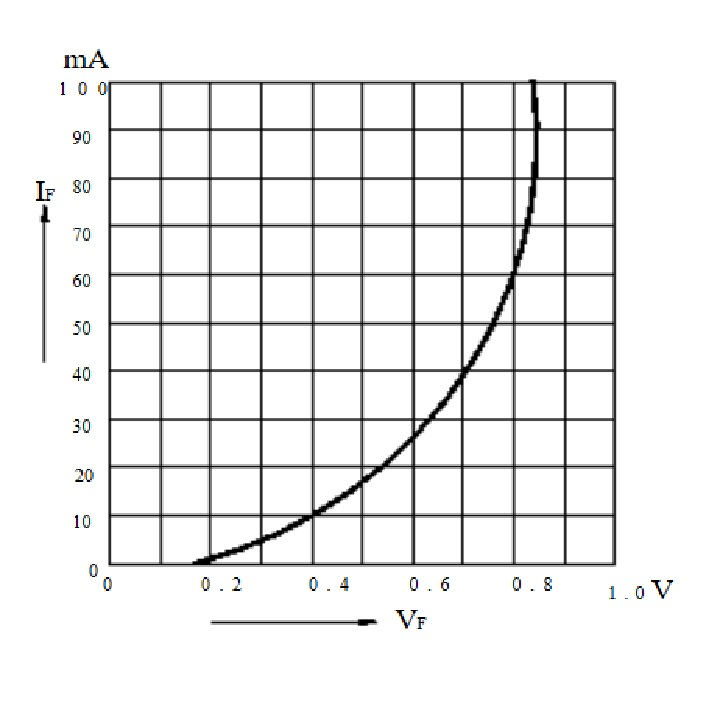
\includegraphics[width=1.1\linewidth]{pictures/Curva_Datash_Ge.jpg}
                                \caption{Grafico de la curva del diodo de Germanio en inversa}
                            \end{minipage}
                        \end{figure}

                        Conociendo los datos que nos brinda el fabricante, sabemos que la tension inversa maxima es de 45$V$, por lo tanto se llega a observar que cerca de ese valor el diodo tiende a la region Zenner.

    \chapter{Actividad de laboratorio}
    
        Se pide poner en practica y corroborar los datos conseguidos en el simulador y armar el mismo circuito propuesto y anotar los valores conseguidos.
        
        \subsection{Diodo de Silicio}
        
  \part{Comportamiento del diodo en función de la temperatura}
    \chapter{Actividad de simulacion}
  \part{Circuitos recortadores con diodos Zener}
    \chapter{Actividad de simulacion}
    \chapter{Actividad de laboratorio}
    \chapter{Analisis sobre parametros de hoja de datos}
\end{document}
